\chapter{Other applications}
\label{chap:applications}

\varan is designed as a flexible framework that can support a variety
of application scenarios involving NVX systems.  In this chaper, we
discuss three such scenarios: transparent failover
(\S\ref{sec:failover}), live sanitization (\S\ref{sec:sanitization}),
multi-version execution (\S\ref{sec:mv-execution}) and record-replay
(\S\ref{sec:record_replay}).

% \subsubsection{Regression Testing}
% \label{sec:testing}

% One of the most obvious applications of \varan framework is regression testing.
% Developers often made various assumption about their programs. When working on
% a new version, regression testing is often used to ensure that these
% assumptions still hold even in the new version. Unfortunately, testing is not
% an exhaustive technique and since regression tests are often written by the
% same developers as the software itself, there is a high probability that some
% violations will be violated leading to security bugs~\todo{Give concrete
% examples.}.

% Executing the regression suite under \varan while running both versions in
% parallel (possibly even more) might help to reveal the subtle differences,
% otherwise undetected by the tests. Our current prototype can be instructed to
% stop the application when a divergence in the event stream is discovered
% providing a detailed information of the difference (\eg system call and its
% arguments). \varan may also attempt to continue execution performing different
% system calls. However, this may not always be possible (\eg in case of network
% communication), see discussion in \ref{sec:patternmatching} for more details.


%The results are summarized in Figure~\ref{fig:scribe_vs_nx}.

%% \begin{figure}[t]
%%   \begin{center}
%%     \caption{Performance comparison.}
%%     \label{fig:scribe_vs_nx}
%%   \end{center}
%% \end{figure}

\section{Transparent Failover}
\label{sec:failover}

%[Cite \cite{rx,fo,mx}]

NVX systems introduce a variety of opportunities for increasing
software reliability and availability via transparent failover.  For
instance, one can run in parallel multiple variants of an application with
different memory layouts, different software revisions or different
implementations of a given interface to survive bugs that occur 
only in some of them.   

\varan makes it easy to implement transparent failover.  When one of the
versions crashes, the \lstinline`SIGSEGV` signal handler installed in each
version notifies the coordinator, which decides what restart strategy
to use.  When one of the followers crashes, the coordinator unsubscribes it
from the list of currently-running followers, and discards it without
affecting other followers.  When the leader crashes, it designates one
of the followers as the new leader (currently the one with the
smallest internal ID), and notifies it to switch its system call table
(\S\ref{sec:rewriting}) to that of the leader, and to restart the last
system call while discarding the old (crashing) leader.

To demonstrate support for transparent failover, we reproduced a
\redis
bug\footnote{\url{https://code.google.com/p/redis/issues/detail?id=344}}
which was also used in the evaluation of \mx~\cite{mx}.  We ran in
parallel eight consecutive revisions of \redis from the range
\lstinline`9a22de8` to \lstinline`7fb16ba`, where the last revision
introduced a bug which crashes the server by causing a segmentation
fault. We then set up a client to send an \lstinline`HMGET` command
that triggers the bug, and measured the increase in latency for that
command.  When the buggy version is a follower, we do not observe any
increase in latency, as expected.  When the buggy version is a leader,
the latency increases from \redisnormallatency to
\redisfailoverlatency.  In both cases, we observed no extra
degradation in throughput for the commands that follow.

%While \mx can
%recover from the crash unlike \varan, which discards the crashing
%version, \mx can only run two versions in parallel while \varan can run
%arbitrary number of versions with significantly lower performance
%overhead as shown in Section~\ref{sec:comparison}.

As an additional experiment, we ran revisions \lstinline`2437` and
\lstinline`2438` of \lighttpd (also used in the evaluation of
\mx~\cite{mx}), the latter of which introduced a crash bug.  We then
set up a client that triggers the bug and measured the latency for
that request. In both cases, \ie when the buggy version was either
the leader or the follower, there was no increase and the latency remained
at \lighttpdnormallatency.
%set up a client that triggers the bug and measured the increase in
%latency for that command. As for the \redis scenario, there is no
%increase in latency when the buggy version is a follower.  When it is
%the leader, the latency increases from \lighttpdnormallatency to
%\lighttpdfailoverlatency.  


\section{Multi-version execution}
\label{sec:mv-execution}

Multiple different software versions (revisions) can be run inside an
NVX system as long as they all issue the same sequence of system
calls~\cite{mx}. This limitation is due to the fact that prior NVX
systems run versions in lockstep (\S\ref{sec:rw}).

Because \varan does not run the versions in lockstep and can use
system call rewrite rules, it can often overcome this limitation. To
illustrate, we used several \lighttpd revisions from the \mx~\cite{mx}
feasibility study which introduced new system calls and as such cannot
be run in parallel by prior NVX systems that rely on lockstep execution.

As a first experiment, we ran revision \lstinline`2435` as
leader together with revision \lstinline`2436` as follower.  Revision
\lstinline`2436` introduces two additional checks using the
\lstinline`getuid` and \lstinline`getgid` system calls.  More
precisely, revisions until and including \lstinline`2435` used
\lstinline`geteuid()` and \lstinline`getegid()` C library functions to
check the user account under which the server is being run, before
issuing an \lstinline`open` system call.  This resulted in a sequence
of \lstinline`geteuid`, \lstinline`getegid` and \lstinline`open`
system calls.  Revision \lstinline`2436` replaced the use of the
aformentioned functions with \lstinline`issetugid()` which changed the
system call sequence to \lstinline`geteuid`, \lstinline`getuid`,
\lstinline`getegid`, \lstinline`getgid`, followed by \lstinline`open`
as before.

To allow for this divergence, we used the custom BPF filter shown in
the Listing~\ref{lst:lighttpd}.  The filter is executed by the
follower whenever a divergence is detected.  In our experiment, this
happens when the follower executes the newly introduced
\lstinline`getuid` system call. The filter first loads the system call
number executed by the leader into the implicit BPF accumulator
(line~\ref{line:load-leader}) and checks whether the call is either
\lstinline`getegid` (line~\ref{line:check-getegid}) or
\lstinline`open` (line~\ref{line:check-open}).  The former will be
true in this case, so the control will transfer to
line~\ref{line:load-getuid}, which loads the system call number
executed by the follower into the accumulator, checks whether it is
\lstinline`getuid` (line~\ref{line:check-getuid}) and finally
transfers the control to line~\ref{line:allow} returning the value
\lstinline`SECCOMP_RET_ALLOW`, which instructs \varan to execute the
additional system call (\ie \lstinline`getuid`) in the follower.  Any
other combination of system calls would have killed the follower
(line~\ref{line:kill}). After executing the \lstinline`getuid` system
call and replaying the execution of \lstinline`getegid` (which the
leader also executed), \varan would detect a second divergence when
the follower tries to execute \lstinline`getgid` instead of
\lstinline`open`. This divergence would be resolved using the same
filter, taking the path on lines~\ref{line:check-open},
\ref{line:load-getgid}, \ref{line:check-getgid} and \ref{line:allow}.

Note this is only one possible filter for allowing this divergence; in
particular, one could write a filter that takes into account more
information about the context in which it should be applied, \eg by
inspecting some system call arguments.

% or more system calls preceding the divergence.


\begin{figure}[t]
\begin{lstlisting}[label={lst:lighttpd},language={[bpf]Assembler},caption={Example of a BPF rewriting rule}]
ld event[0] /*@\label{line:load-leader}@*/
jeq #108, getegid       /* __NR_getegid *//*@\label{line:check-getegid}@*/
jeq #2, open            /* __NR_open *//*@\label{line:check-open}@*/
jmp bad
getegid:
ld [0]                  /* offsetof(struct seccomp_data, nr) *//*@\label{line:load-getuid}@*/
jeq #102, good          /* __NR_getuid *//*@\label{line:check-getuid}@*/
open:
ld [0]                  /* offsetof(struct seccomp_data, nr) *//*@\label{line:load-getgid}@*/
jeq #104, good          /* __NR_getgid *//*@\label{line:check-getgid}@*/
bad: ret #0             /* SECCOMP_RET_KILL *//*@\label{line:kill}@*/
good: ret #0x7fff0000   /* SECCOMP_RET_ALLOW *//*@\label{line:allow}@*/
\end{lstlisting}
\end{figure}

%% To translate the filter into bytecode, the user can use the provided
%% \lstinline`vx_bpf` tool and pass the output directly to \varan when starting the
%% application:

%% \begin{lstlisting}[language={bash},numbers=none]
%% vx --filter "$(vx_bpf lighttpd.filter)" \
%%   /path/lighttpd-2435 /path/lighttpd-2436 \
%%   -- -f lighttpd.conf
%% \end{lstlisting}

We used a similar filter to run revisions \lstinline`2523` and
\lstinline`2524`, the latter of which introduces an additional
\lstinline`read` system call to access the \lstinline`/dev/urandom`
file to obtain an additional source of entropy.  We were also able to
run revisions \lstinline`2577` and \lstinline`2578` where the
difference consists of an additional \lstinline`fcntl` system call to
set a \lstinline`FD_CLOEXEC` flag on one of the file descriptors.

Currently, \varan's implementation can use BPF filters to allow adding
or removing system calls in the follower.  However, this is not a
fundamental limitation, and in the future we plan
%to use the powerful pseudo-machine model employed by BPF filters
to support  other types of transformations, such as replacing one
sequence of system calls with another.

%% The BPF rewrite rules can be used to handle one-to-many and many-to-one
%% situations (\ie where a single system call has been replaced by multiple ones)
%% as shown in Section~\ref{sec:mv-execution}, but they are not suitable for
%% many-to-many scenarios, mainly due to limited expressive power of the language.
%% This issue could be addressed in the future by the use of more expressive
%% language such as eBPF.


%We managed to ran \lighttpd revision \lstinline`2435` together with
%the following revision \lstinline`2436`, which introduced two extra
%checks using the system calls \lstinline`getuid` and
%\lstinline`getgid`. We configured \varan to allow followers to skip
%these calls, or conversely to execute them if they are not found in
%the event stream, using the custom BPF filter shown in the
%Listing~\ref{lst:lighttpd}.

% \begin{figure}[t]
% \begin{lstlisting}[label={lst:lighttpd},language={[bpf]Assembler},caption={Example of a BPF rewriting rule}]
% ld #syscall
% jneq #2, bad            /* __NR_open */
% jneq #108, bad          /* __NR_getegid */
% ld [0]                  /* offsetof(struct seccomp_data, nr) */
% jeq #102, good          /* __NR_getuid */
% jeq #104, good          /* __NR_getgid */
% jeq #107, good          /* __NR_geteuid */
% jeq #108, good          /* __NR_getegid */
% bad: ret #0             /* SECCOMP_RET_KILL */
% good: ret #0x7fff0000   /* SECCOMP_RET_ALLOW */
% \end{lstlisting}
% \end{figure}

%% To translate the filter into bytecode, the user can use the provided
%% \lstinline`vx_bpf` tool and pass the output directly to \varan when starting the
%% application:

%% \begin{lstlisting}[language={bash},numbers=none]
%% vx --filter "$(vx_bpf lighttpd.filter)" \
%%   /path/lighttpd-2435 /path/lighttpd-2436 \
%%   -- -f lighttpd.conf
%% \end{lstlisting}

% When \varan detects the divergence in the follower, it runs the filter
% to try to resolve the divergence. Since the provided filter matches
% the input and returns the \lstinline`SECCOMP_RET_ALLOW` value, \varan
% executes the additional system calls in the follower.  After these
% calls, the execution continues as expected, with both versions issuing
% the same system call sequence.

% As a second experiment, we ran \lighttpd revision \lstinline`xxx` with
% the following revision \lstinline`xxx+` which introduced an extra
% \lstinline`read` call to \lstinline`/dev/[u]random`.  We wrote a BPF
% filter similar to the one before, which allows followers to skip this
% call, or conversely to execute it if it is not found in the event
% stream. The filter allows the divergence to be resolved, after which
% both versions continue to issue the same system call sequence.

%% As a second experiment, we ran \lighttpd revision \lstinline`xxx` with

% \lighttpd: a pair of \lstinline`geteuid()` and \lstinline`getegid()`
% calls are replaced with a single call to \lstinline`issetugid()`.


%To handle various instances of these classes, we introduced an approach
%based on pattern matching. The pattern language employed by \varan is
%similar to regular expressions, but rather than instances of strings, it
%is used to match instances of system call traces. We have employed
%regular language which allows us to construct a non-deterministic finite
%automaton for each pattern using the technique introduced by Ken
%Thompson~\cite{regexp}.

%The pattern language employed by also \varan allows to match system call
%arguments, similarly to BPF filters in mode 2 seccomp provided by Linux
%kernel, which is necessary to match certain traces.



% and restarts the last system call.  All other followers simply discard
% the event and continue in execution.

% and then notifies all versions by issuing a special
% "reranking" event and sends new ranks to all instances over the
% service channel. When the event is read by individual followers during
% replay, they receive their new ranks and take the action. 


% \todo{Memory consumption?}

% \begin{structure}
% \item Scaling w/ more versions/variants
% \item Fail-over mechanism w/ many versions/variants
% \item Multiple versions: \mx, staged deployment
% \item Variants: sanitizers? some memory allocation diffs?
% \item different compilers?  gcc vs llvm?
% \item sanitizers?
% \end{structure}

\section{Live Sanitization}
\label{sec:sanitization}

\begin{figure}[t]
  \begin{center}
    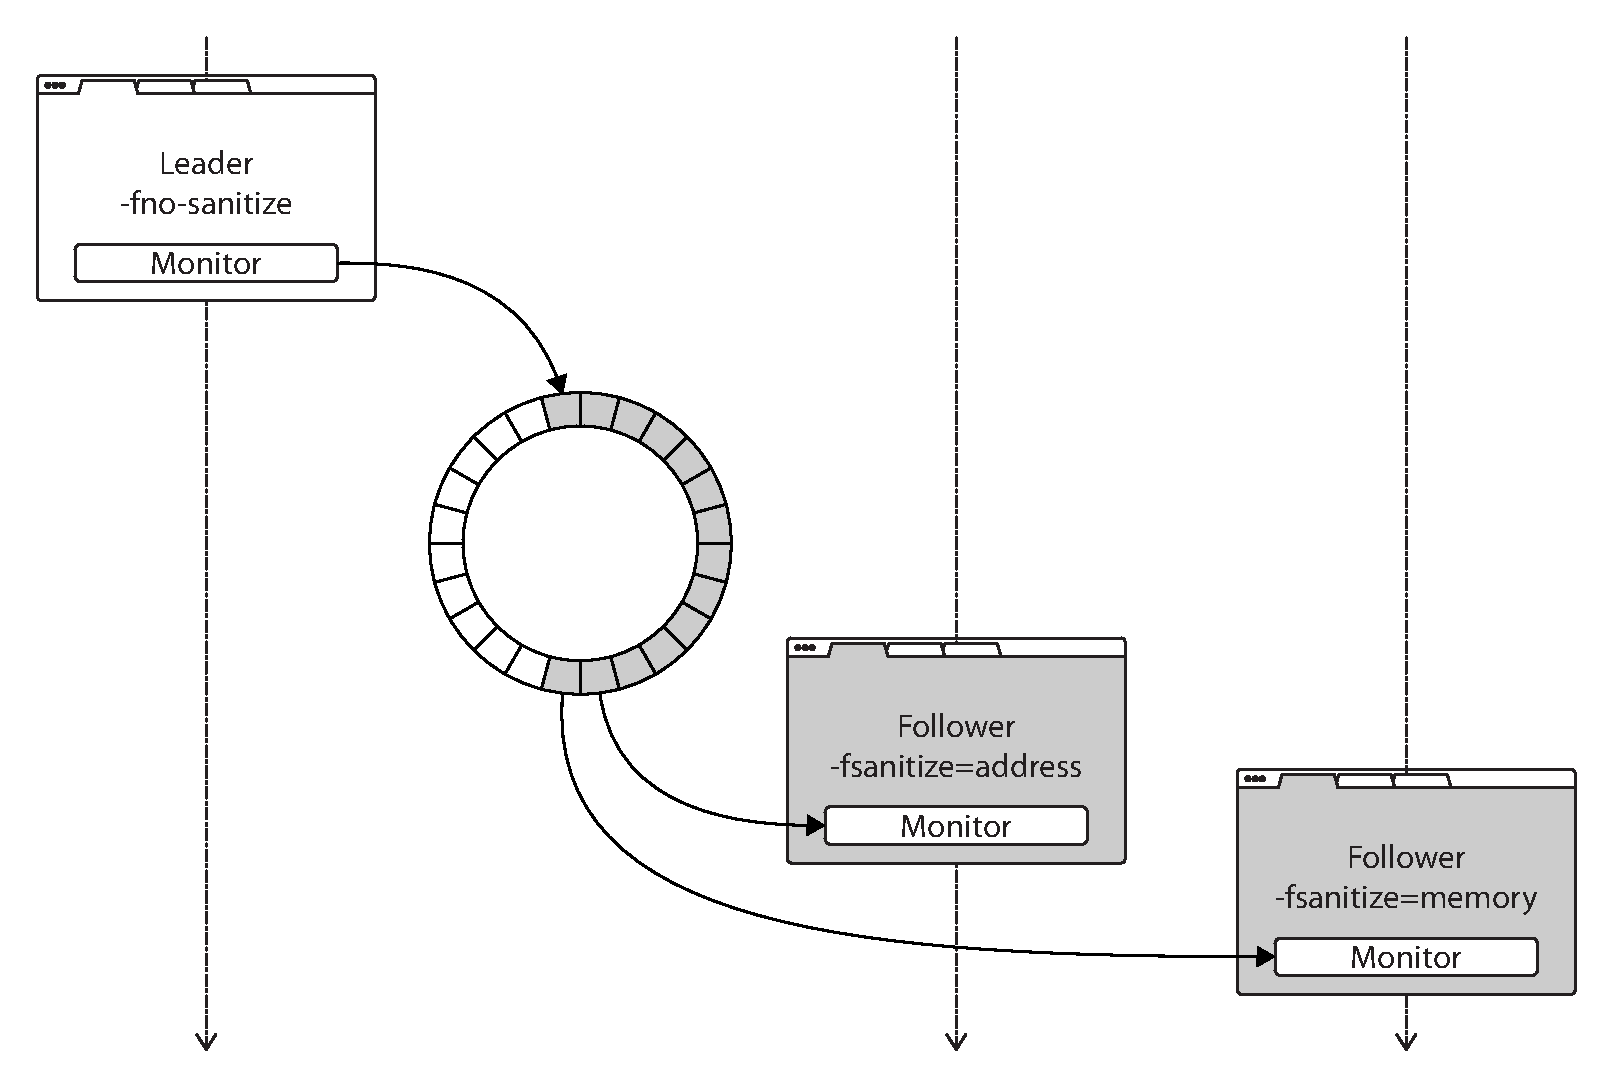
\includegraphics[width=0.75\columnwidth]{applications/figures/live-sanitization}
    \caption{The use of event-streaming architecture for live sanitization.}
    \label{fig:live-sanitization}
  \end{center}
\end{figure}

Sanitization is one of the most effective testing techniques for
revealing low-level bugs such as uninitialized pointer dereferences and
use-after-free errors.  Both Clang and GNU C Compiler now include a set
of sanitizers---AddressSanitizer (ASan), MemorySanitizer (MSan),
ThreadSanitizer (TSan)---which can be used to statically instrument
the code with various checks.  Unfortunately, these checks introduce
extra overhead (\eg $~2\times$ for ASan, $~3\times$ for MSan and
$~5$-$15\times$ for TSan).  which is why these sanitizers are typically
only used in off-line testing. However, during testing developers only
use a limited set of inputs which might not reveal all bugs.

One possible solution is to record execution traces during deployment
and then replay them in a testing environment with sanitization
enabled. However, this approach is unlikely to work in practice for
several reasons. First, since we do not know in advance which traces
are potentially interesting (\eg trigger sanitization checks) and
which are not, we have to potentially collect and replay a huge number
of execution traces. Even with some form of deduplication, this is
usually impractical. Second, for long-running applications such as
servers, the log size will quickly grow to a large size. Third, many
customers will refuse to share the logs from their production
deployment.
% While we may attempt to anonymize these logs, this could
% potentially hide interesting cases.

With \varan, we can perform live sanitization by running the native
unsanitized version as the leader, with sanitized versions as
followers.%, as shown in Figure~\ref{fig:live-sanitization}.
While sanitization itself introduces a performance overhead, since
followers do not need to execute any I/O operations and merely replay
them, they can often keep up with the leader, allowing users to run
sanitized versions in production without introducing any significant
overhead.

To demonstrate this, we build revision \lstinline`7f77235` of \redis
twice: once with Clang without any sanitization, once with ASan
enabled.  We then ran both versions in parallel using \varan and used
the same benchmark with the same settings as for our performance
evaluation (\S\ref{sec:c10k}). As expected, we have not measured any
additional slowdown in the leader compared to the scenario with two
non-sanitized versions being run in parallel. To get a better insight
into the effect of running the sanitized version with \varan, we have
measured the median length of the log, \ie the distance between the
leader and the follower. With sanitization, this length increases from
\redisNoSanitizationMedianLength to \redisSanitizationMedianLength,
which does not impose any problems.

\section{Record-Replay}
\label{sec:record_replay}

Although \varan shares similarities with record-replay systems, there are
significant differences; in particular, the log is of fixed size and
only kept in-memory.  However, it is possible to easily extend \varan to
provide full record-replay capabilities by implementing two artificial
clients:
\begin{inparaenum}[(i)]
\item one acting as a \emph{follower} whose only goal is to write the
  content of the ring buffer to persistent storage, and
\item one acting as a \emph{leader}, reading the content of the log
  from the persistent storage and publishing events into the ring
  buffer for consumption by other clients.
\end{inparaenum}

Compared to some of the previous record-replay systems, \varan has a
number of advantages. First, decoupling the logic responsible for
reading/writing the log from the actual application into a separate
process allows the application to run at nearly full speed and utilize
the multiple cores available in modern CPUs.  Second, since \varan was
designed to run multiple instances at the same time, we can replay
multiple versions at once, \eg to determine which versions of the
application from a given range are susceptible to a crash reported by
the user.

We have implemented a simple prototype of the two aforementioned
clients on top of \varan and compared its performance against
\scribe~\cite{scribe}, a state-of-the-art record-replay system
implemented in the kernel.  Unfortunately, because \scribe is
implemented in the kernel and is only maintained for an old 32-bit
Linux kernel (2.6.35), we had to run our experiments inside a virtual
machine (kindly provided to us by \scribe's authors, as the source tree
was broken at the time of our experiments). 
%% This experience clearly shows one of the main disadvantages of
%% kernel-level frameworks---the difficulty of maintaining the code base.
To allow for a more faithful comparison, we ran \varan inside the same
virtual machine.

We used \redis as a benchmark, running the same workload as before,
and configured both systems to record the execution to persistent
storage.  We recorded an overhead of \redisRROvhScribe for
\scribe,\footnote{The overhead we measured for \scribe is higher than
  the overhead reported in~\cite{scribe}; however, note that the original
  work used less aggressive benchmarks such as \httpd.  The use of a
  virtual machine also affected the result.}  compared to
\redisRROvhNx for \varan.
%(but remember that we ran it inside a virtual machine)

% Despite being implemented in the kernel, \scribe
% performed worse than \varan on our \redis experiments: the overhead
% introduced by \scribe was \redisRROvhScribe, compared to only
% \redisRROvhNx for \varan.

\section{Honeypots}
\section{Testing}
